\documentclass[a4paper, 12pt, titlepage]{article}

% Including needed packages
\usepackage[margin=2cm]{geometry}
\usepackage{amsmath}
\usepackage{bbm}
\usepackage{graphicx}
\usepackage{subfig}
\usepackage{float}

\title
{{\em Machine learning lab course}\\
Problem set 2: Clustering, EM}
\author{ROHRMANN Till, Matrnr: 343756\\
\texttt{till.rohrmann@campus.tu-berlin.de}}
\date{\today}

\begin{document}

\maketitle

\part{Introduction}
\label{part:introduction}

The second problem set dealt with the clustering problem.
Clustering analysis is the problem to find groups of data points which which are more similar to each other than to data points of other groups.
This plays an important role in a wide variety of fields such as machine learning, bioinformatics and data mining for example.

In the context of the work, I implemented and evaluated three different clustering algorithms:
\texttt{k-means} as a representative of a centroid model, \texttt{hierarchical clustering} as a representative of a connectivity model and \texttt{EM algorithm} as a representative of distribution models.
The evaluation was done by clustering provided test data sets and investigating how well the different groups have been found.

The report is structured as follows:
In part \ref{part:implementation} I will explain shortly the subtlenesses of the implementation and the encountered pitfalls while coding the algorithms.
In part \ref{part:appliation} the implemenations are applied to the test data sets.
The interpretation of the results and the performance evaluation is given in this part as well.

\part{Implementation}
\label{part:implementation}

One problem I encountered while implementing the hierarchical clustering was that the \texttt{mergeidx} return value of \texttt{kmeans\_agglo} did not work properly with the function \texttt{scipy.cluster.hierarchy} \texttt{.dendrogram}.
In order to fix it, I changed slightly the semantic of \texttt{mergeidx}.
The array \texttt{mergeidx} is a $k-1 \times 2$ vector with $k$ being the number of initial clusters which shall be merged.
\texttt{mergeidx[i][0]} and \texttt{mergeidx[i][1]} contain the identifier of the clusters which are merged in the $i$th step.
But instead of giving the newly merged cluster the index \texttt{mergeidx[i][1]}, a new index $k+i$ is introduced and assigned to the cluster.
However, this change does not affect the overall semantics of the algorithm.

A problem of the \texttt{EM algorithm} is a possible overfitting of a mixture component to one data point.
Since one maximizes the likelihood of the Gaussian mixture components, it might be possible that one component is centered on one data point.
By letting the covariance matrix converge to $0$, the overall likelihood increases to $\infty$.
One can prevent that from happening by regularizing the estimated covariance matrices:

\begin{eqnarray*}
	CovMatrix &=& \frac{(\hat X-\mu)(\hat X-\mu)^T)}{\mathbbm{1}^T\gamma} + \delta\cdot Id
\end{eqnarray*}

Where $(\gamma)_i$ is the probability of the data point $x_i$ belonging to the cluster $\mu$, the columns of $\hat X$ are $\sqrt{(\gamma)_i}\cdot x_i$ and $\delta$ is the regularization constant.

Furthermore, while running the expectation-maximization clustering on the test data set \texttt{USPS}, I encountered such small determinants of the covariance matrices while computing the probability density function which lead to cancellation and consequently causing the algorithm to fail.
In order to cope with those problems, one could have increased the regularization constant of the covariance matrices and thus preventing a too small probability.
However, I decided to go another way and implemented the algorithm executing its calculations in the log space.
By taking the log of a probability and calculating with those values, we can avoid the numerical problems of really small determinants.
But nothing comes for free.
While products become sums in the log space, sums have to be treated differently.
A numerically stable variant is the following.
Given to variables $a$ and $b$ of which we want to calculate the sum in log space.

\begin{eqnarray*}
	\log \left( a+b \right) &=& \log a + \log \left(1+\frac{b}{a}\right)\\
	&=& \log a  + \log \left(1+ \exp\left( \log b - \log a \right) \right)
\end{eqnarray*}

Assuming that $a>b$, gives us now a numerically stable sum operation in the log space. 

For further details see the implementations in the file \texttt{ps2\_implementation.py}.

\part{Application}
\label{part:application}

\section{Assignment 6}

In this assignment, we were supposed to apply the \texttt{k-means}, the \texttt{EM-algorithm} and the \texttt{hierarchical clustering} onto the data set \texttt{5gaussians}.
This data set contains $500$ $2$-dimensional data points sampled from a Gaussian mixture distribution.
The distribution consists of 5 components with different means and covariance matrices.
\begin{figure}
	\centering
	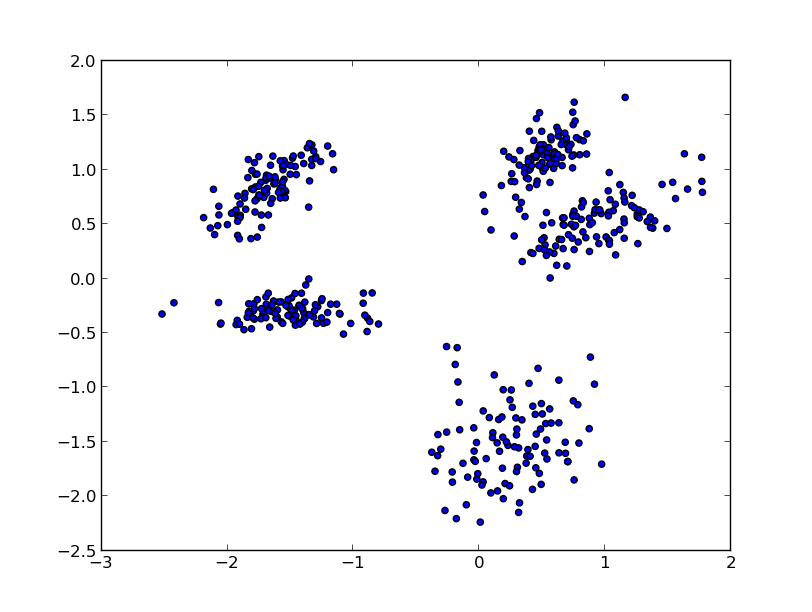
\includegraphics[width=12cm]{images/5gaussians.png}
	\caption{Scatter plot showing the data set \texttt{5gaussians}.}
	\label{fig:5gaussians}
\end{figure}
A scatter plot of the initial data can be seen in Figure \ref{fig:5gaussians}.
The distinct Gaussian distributions can be clearly seen.

Since it is apriori not known how many clusters a data set contains, the analysis is run for the number of clusters $k=2,\ldots,10$.
The \texttt{k-means} algorithm was executed with a maximum iterations of $500$.
The \texttt{EM-algorithm} was run as well with a maximum iterations of $500$.
Additionally, the regularization constant was set to $\delta = 1e-5$ and the termination threshold of the log-likelihood to $\epsilon = 1e-3$.
That is to say, as soon as the log-likelihood between the current iteration and the preceding iteration surpasses this threshold, the iteration procedure is stopped.
Furthermore, I investigated the influence of a preceding initialization with \texttt{k-means} of the \texttt{EM-algorithm} on the obtained results.
Since I did not encounter any numerically problems with this data set, I used the \texttt{EM-algorithm} implementation which calculates in the normal space (see \texttt{em\_mog}).
Since the algorithms strongly depend on the initialization, the performance as well as the result, I executed all algorithms $30$ times and took the result with minimal error and maximum log-likelihood, respectively.
The $30$ runs are also used to calculate the average number of iterations and the average time per iteration needed.

The error function for the \texttt{k-means} algorithm is simply the sum of the distances of each data point to its assigned cluster.
For the \texttt{EM-algorithm} it is the sum of the distances of each data point to all clusters weighted by its membership probability of a cluster:

\begin{eqnarray*}
	Error_{EM} &=& \sum_{i=1}^N \sum_{j=1}^k \gamma_{i,j} \sqrt{\lVert X_i-\mu_j \rVert_2}
\end{eqnarray*}

\begin{figure}
	\centering
	\subfloat{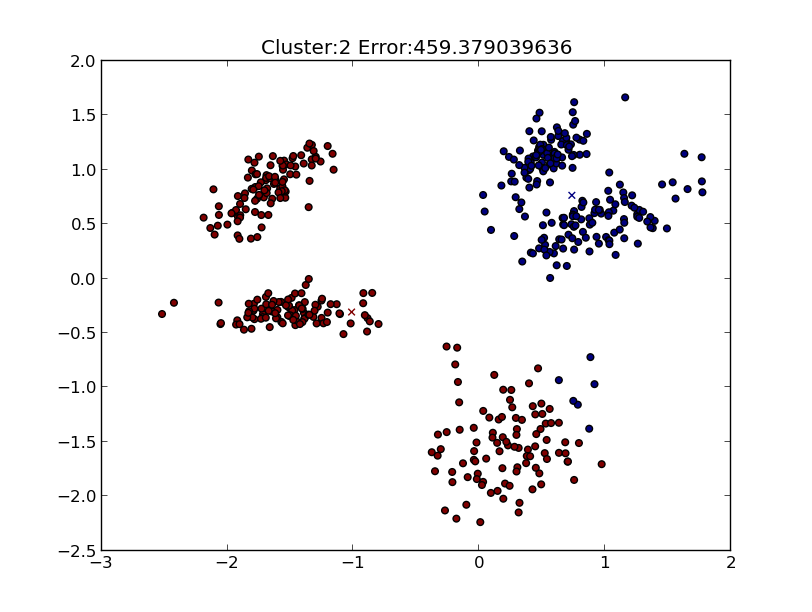
\includegraphics[width=6cm]{images/km2.png}}
	\subfloat{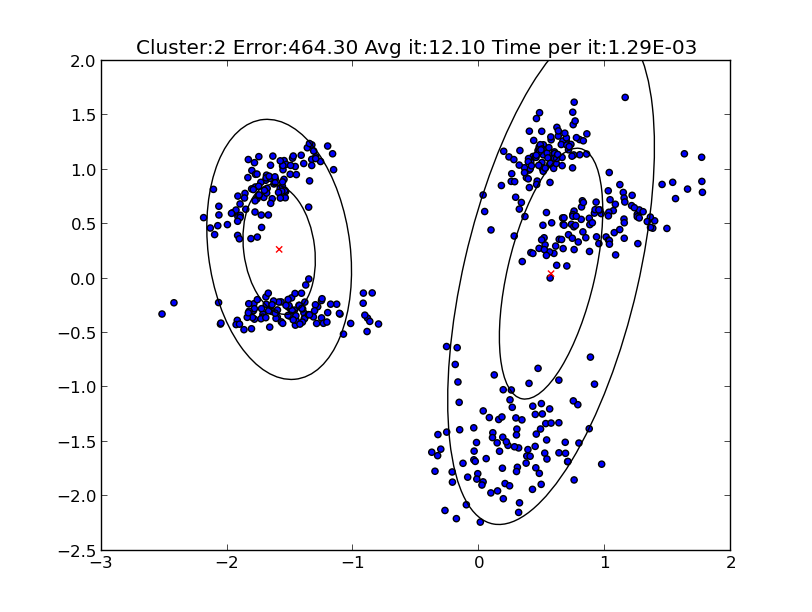
\includegraphics[width=6cm]{images/em2.png}}
	\subfloat{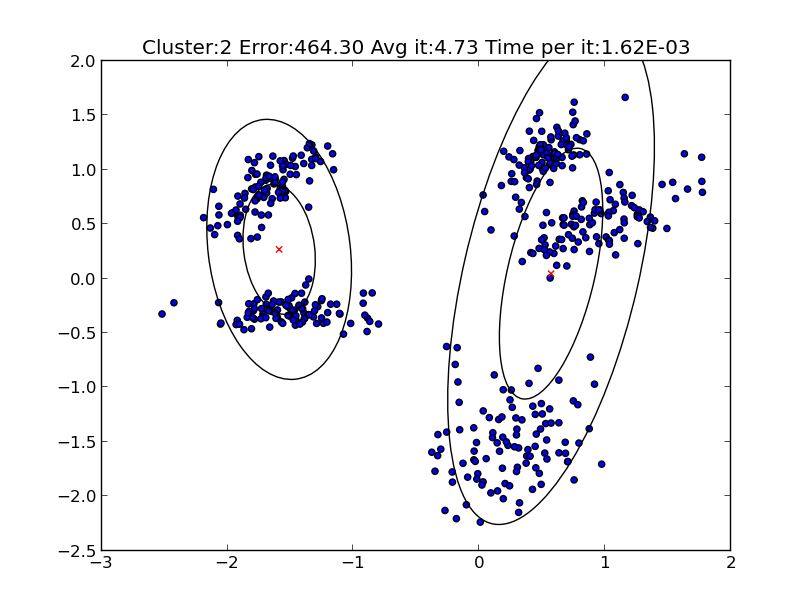
\includegraphics[width=6cm]{images/em2km.png}}\\
	\subfloat{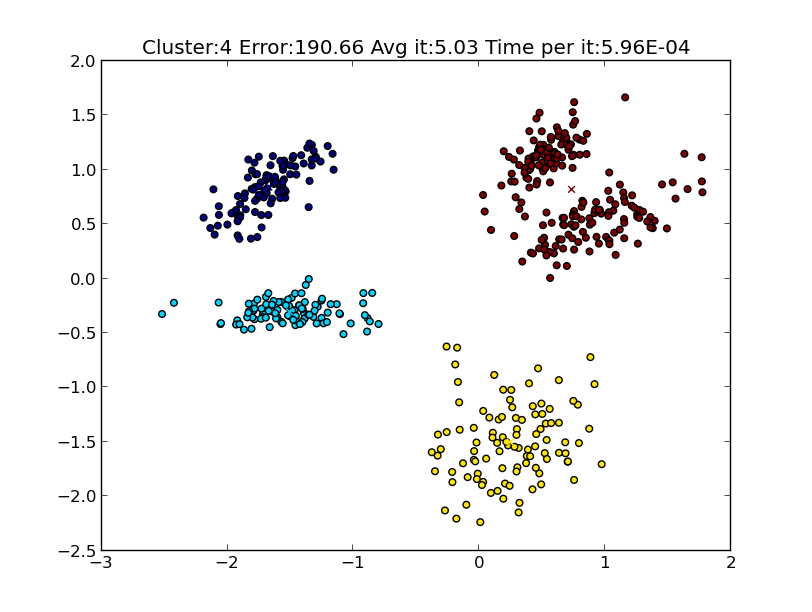
\includegraphics[width=6cm]{images/km4.png}}
	\subfloat{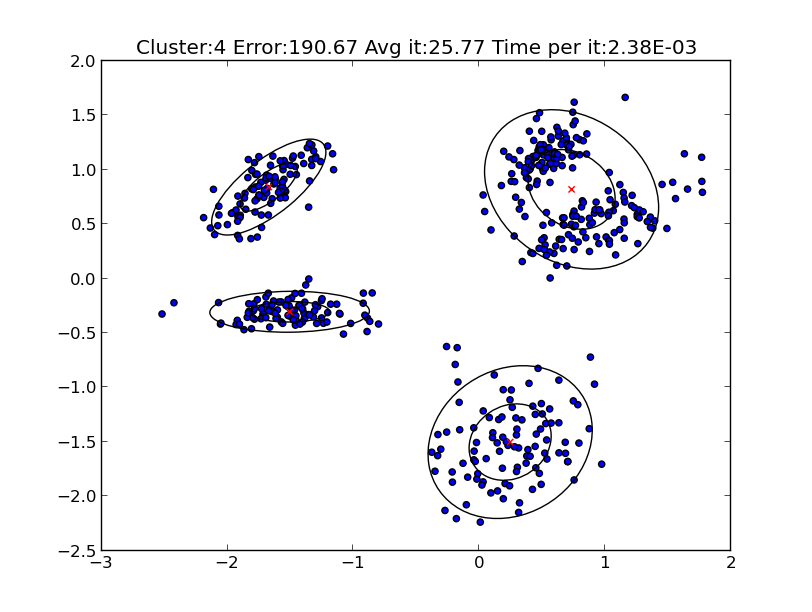
\includegraphics[width=6cm]{images/em4.png}}
	\subfloat{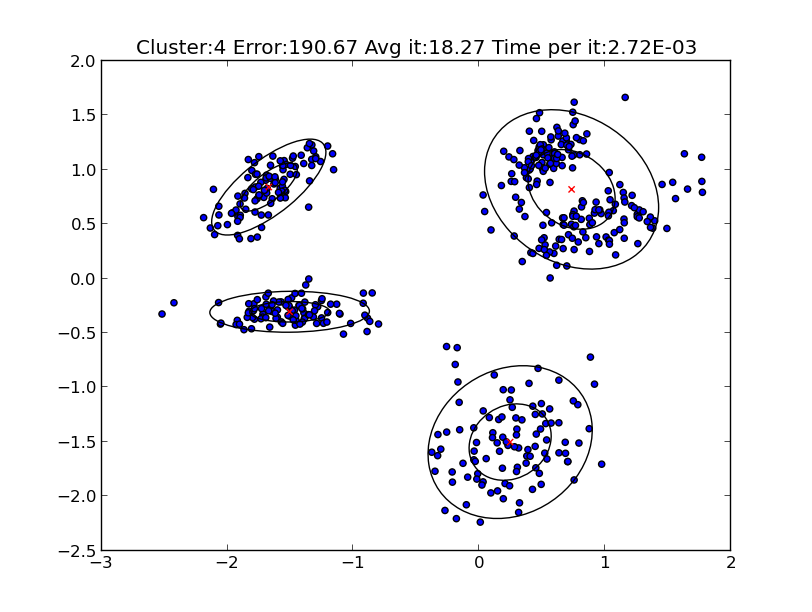
\includegraphics[width=6cm]{images/em4km.png}}\\
	\subfloat{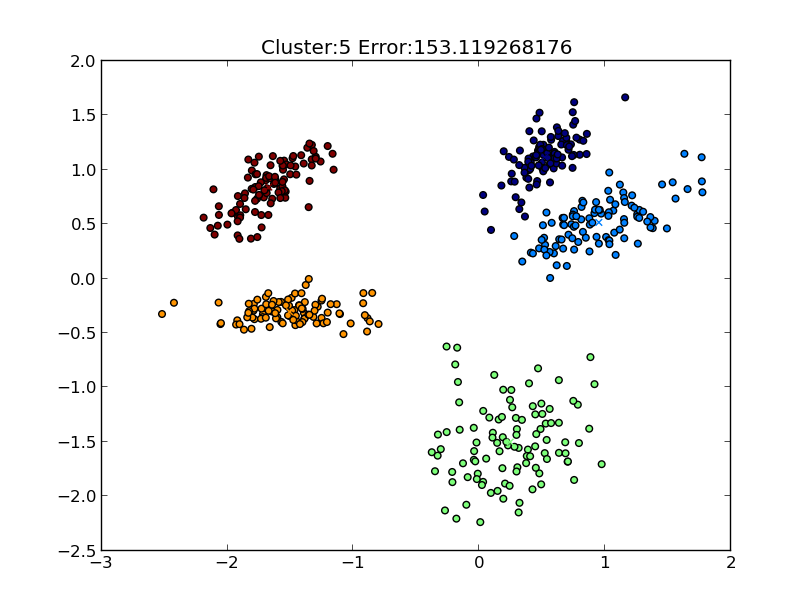
\includegraphics[width=6cm]{images/km5.png}}
	\subfloat{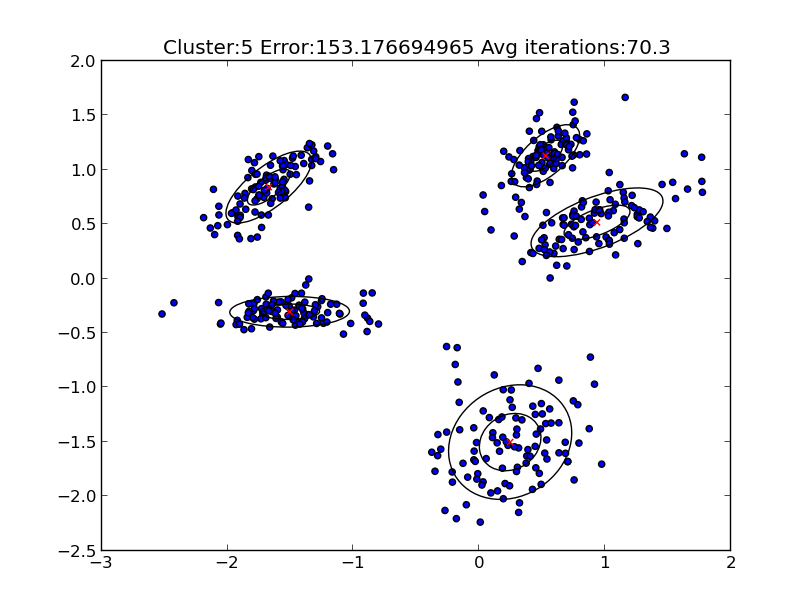
\includegraphics[width=6cm]{images/em5.png}}
	\subfloat{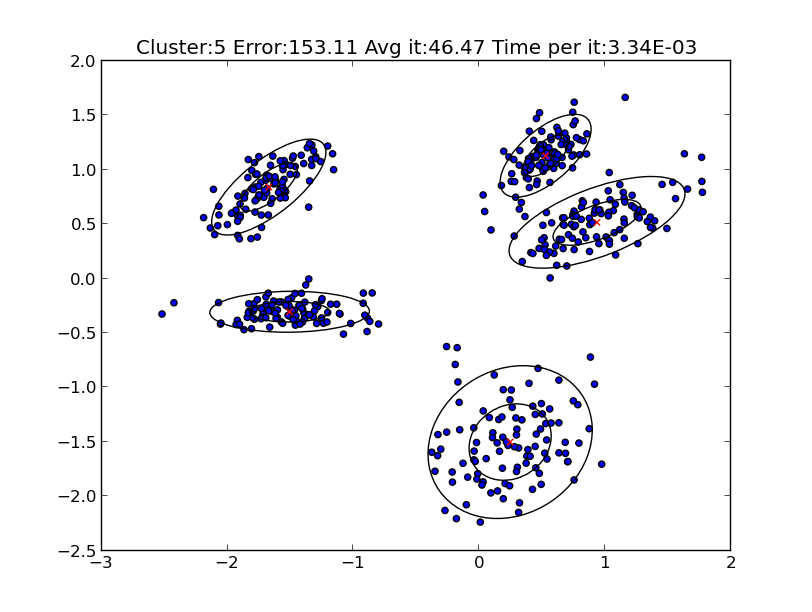
\includegraphics[width=6cm]{images/em5km.png}}\\
	\subfloat{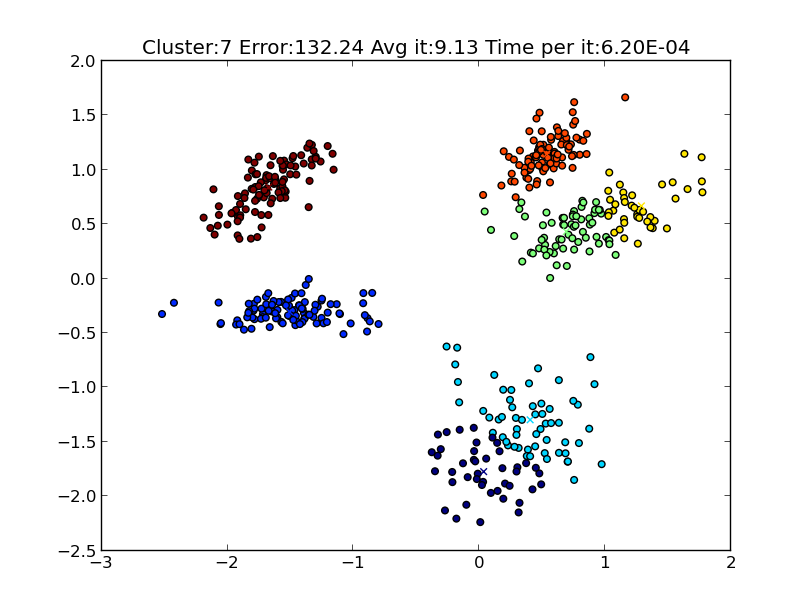
\includegraphics[width=6cm]{images/km7.png}}
	\subfloat{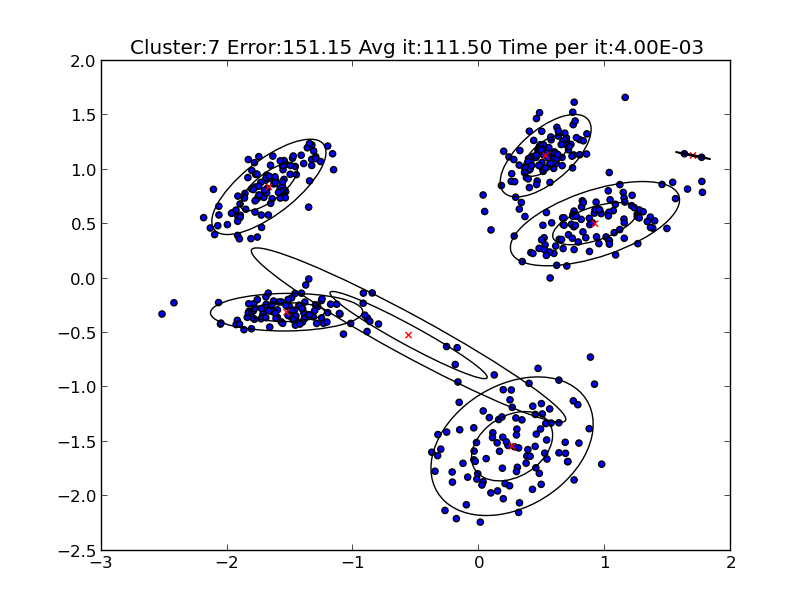
\includegraphics[width=6cm]{images/em7.png}}
	\subfloat{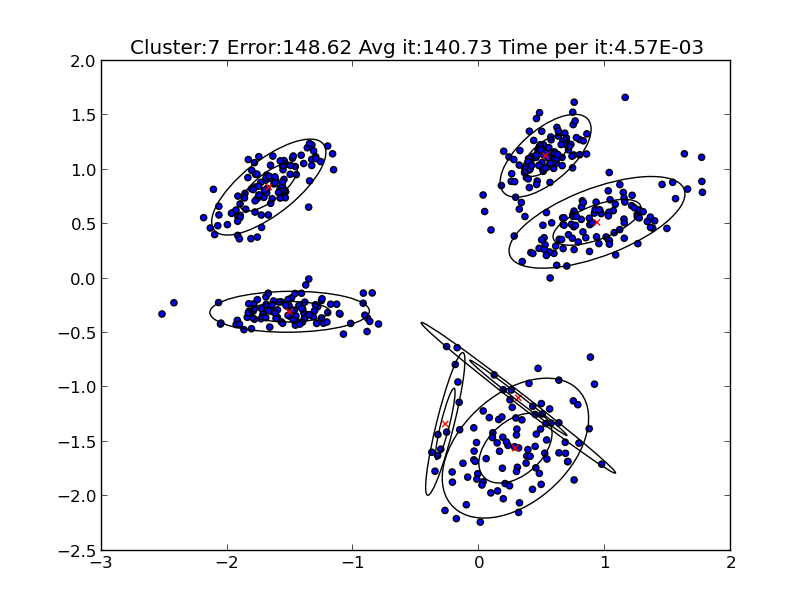
\includegraphics[width=6cm]{images/em7km.png}}
	\caption{Results of clustering analysis for a subset of cluster numbers. Left column: Results of \texttt{k-means}. Middle column: Results of \texttt{EM-algorithm} without initialization. Right column: Results of \texttt{EM-algorithm} with \texttt{k-means} initialization. First row: $2$ clusters, second row: $4$ clusters, third row: $5$ clusters and fourth row: $7$ clusters.}
	\label{fig:5gaussiansClustering}
\end{figure}

\subsection{Do \texttt{k-means} and the \texttt{EM-algorithm} find the 5 clusters reliably?}

In Figure \ref{fig:5gaussiansClustering} one can see a selection of clustering results of the algorithms \texttt{k-means} and \texttt{EM-algorithm} for different numbers of clusters.
Especially the third row is interesting, because it contains the result with the correct number of clusters, that is to say $5$.
Here we can see that all variants find reliably the 5 clusters.
For the \texttt{k-means} the different clusters are color-coded while the Gaussian mixture model is indicated by the covariance ellipses around the mean at the distance one time and two times the standard deviation.
Furthermore, we can observe a deviating behavior of the two algorithms for a cluster number higher than $5$.
As we can see in the last row of Figure \ref{fig:5gaussiansClustering}, the \texttt{k-means} algorithm successfully sub-divides the individual clusters into the half.
In contrast, the \texttt{EM-algorithm} finds additional Gaussians mixture components which seem to be highly degenerated, that is to say they have a covariance matrix with a highly dominating eigenvalue.

In order to evaluate the performance of the different algorithms, I plotted in Figure \ref{fig:5gaussiansError} the error with respect to the number of clusters, in Figure \ref{fig:5gaussiansIterations} the number of iterations until convergence and in Figure \ref{fig:5gaussiansTime} the total number of time needed until convergence.

\begin{figure}
	\centering
	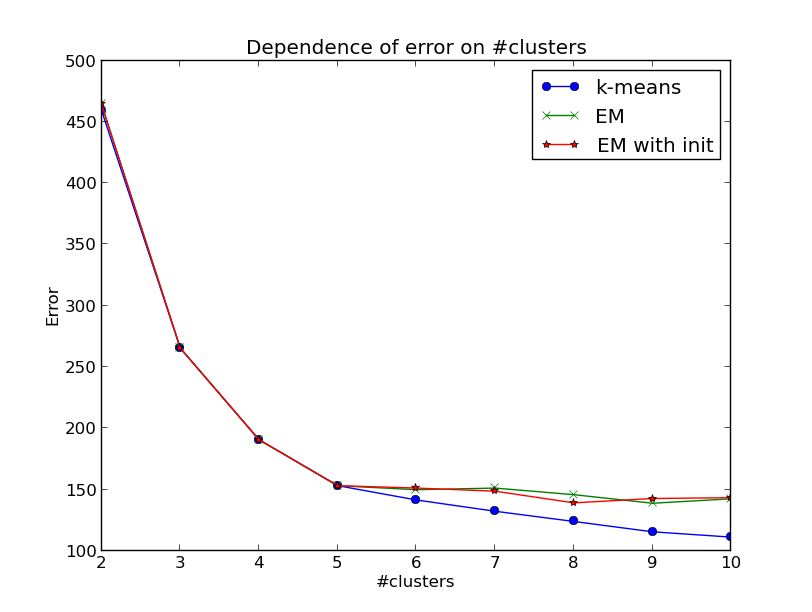
\includegraphics[width=8cm]{images/5gaussiansError.png}
	\caption{Error of clustering of \texttt{k-means}, \texttt{EM-algorithm} without and \texttt{EM-algorithm} with initialization with respect to the number of clusters.}
	\label{fig:5gaussiansError}
\end{figure}

\begin{figure}
	\centering
	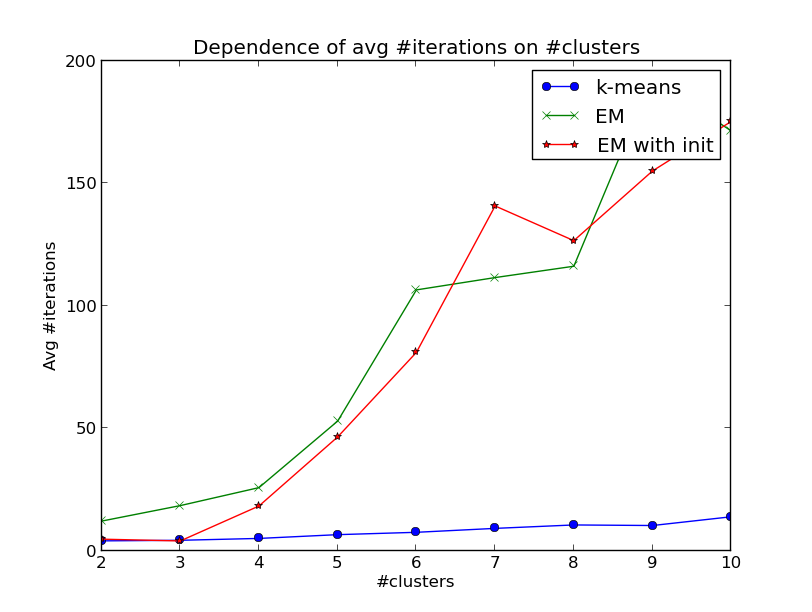
\includegraphics[width=8cm]{images/5gaussiansIterations.png}
	\caption{Number of iterations until convergence of \texttt{k-means}, \texttt{EM-algorithm} without and \texttt{EM-algorithm} with initialization with respect to the number of clusters.}
	\label{fig:5gaussiansIterations}
\end{figure}

\begin{figure}
	\centering
	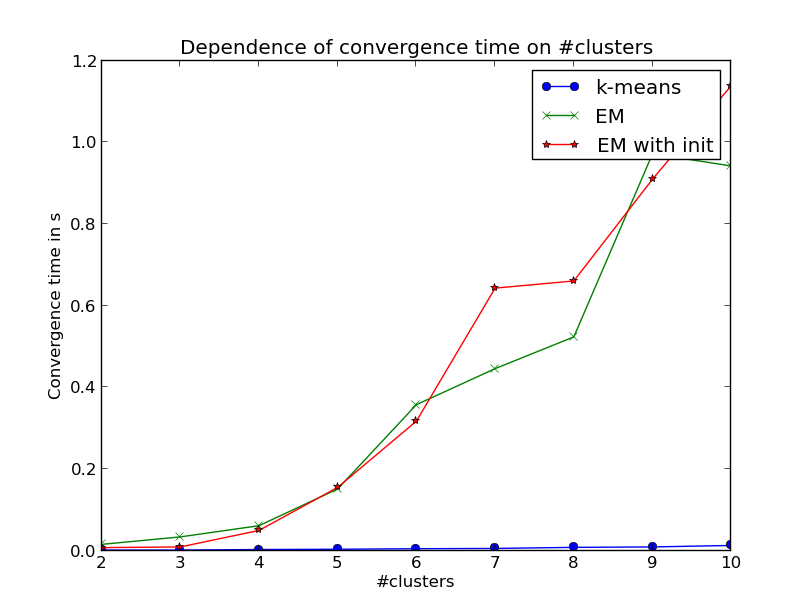
\includegraphics[width=8cm]{images/5gaussiansTime.png}
	\caption{Total time until convergence of \texttt{k-means}, \texttt{EM-algorithm} without and \texttt{EM-algorithm} with initialization with respect to the number of clusters.}
	\label{fig:5gaussiansTime}
\end{figure}

We can see in Figure \ref{fig:5gaussiansError} that the \texttt{k-means} algorithm performs best.
It is noteworthy that the error of the \texttt{EM-algorithm} with and without initialization stays almost constant for more than $5$ clusters.
This illustrates the incapability of the \texttt{EM-algorithm} to further discriminate the clusters.
In Figure \ref{fig:5gaussiansIterations} we can observe that the number of iterations of \texttt{k-means} increases only slowly with increasing number of clusters compared to the \texttt{EM-algorithms}.
For the \texttt{EM-algorithms} we can see that the average number of iterations until convergence increases quickly with the number of clusters.
If we take a look at the total time needed for the computation in Figure \ref{fig:5gaussiansTime}, the same observation can be made.
While the \texttt{k-means} runtime increases slowly the \texttt{EM-algorithms}' runtime increases rapidly.
In fact, the average time for one iteration of \texttt{k-means} is one magnitudes faster than an iteration of the \texttt{EM-algorithm}.
This shows quite well that the \texttt{k-means} algorithm is superior to the \texttt{EM-algorithms} for the \texttt{5gaussians} data set.
The result is not really surprising considering the more complex computations involved in the \texttt{EM-algorithm}.

\subsection{What role does the initialisation of the \texttt{EM-algorithm} play?}

In Figure \ref{fig:5gaussiansError} we can observe that the \texttt{EM-algorithm} with initialization does not necessarily benefit from the \texttt{k-means} initialization in terms of accuracy if one runs the version without initialization often enough (here $30$ times).

However, the convergence rate benefits from the \texttt{k-means} initialization step.
A preceding \texttt{k-means} initialization speeds the \texttt{EM-algorithm} noticeably up if the number of clusters is smaller or equal to the real number of clusters.
However, once exceeded the real number of clusters, a prior initialization does not guarantee to improve the convergence rate.
In that case, we see clearly in Figure \ref{fig:5gaussiansIterations} that the \texttt{EM-algorithm} with initialization performs sometimes better and sometimes worse than the same version without initialization.
If we take a look at the convergence time, we can observe a similar behavior: The initialized \texttt{EM-algorithm} performs first better than the non initialized version if the number of clusters is smaller or equal to $5$.
If the number of assumed clusters is higher than $5$, an initialization does not necessarily speed the convergence time up.

\subsection{What does the dendrogramm of the hierarchical clustering look like?}

\begin{figure}
	\centering
	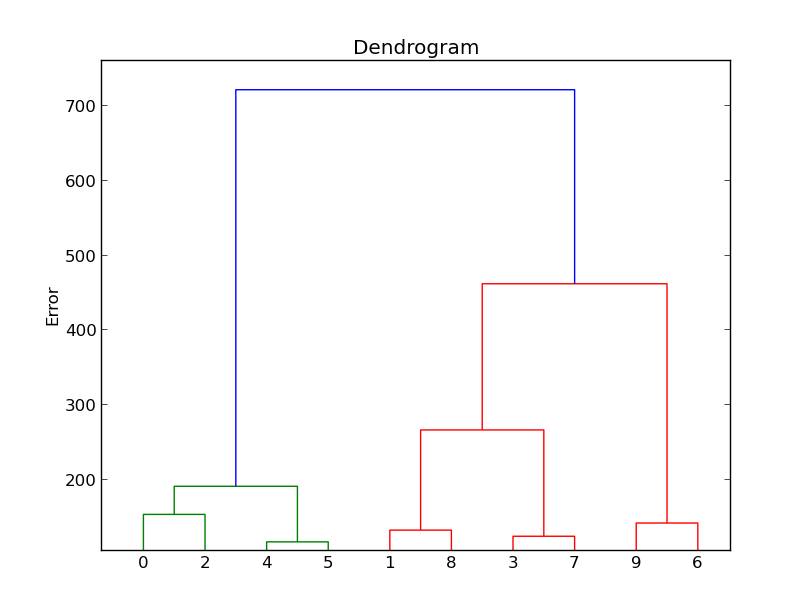
\includegraphics[width=8cm]{images/dendrogram5Gaussians.png}
	\caption{Dendrogram of the hierarchical clustering of the data set \texttt{5gaussians}.}
	\label{fig:dendrogram5Gaussians}
\end{figure}

In Figure \ref{fig:dendrogram5Gaussians} we can see the dendrogram of the hierarchical clustering algorithm which has initially started with 10 clusters.
Estimating the number of cluster $k$ from the dendrogram, I would have chosen $k=4$.
The reason for that is that there is jump of almost $50\%$ of the preceding error.

\section{Assignment 7}

In this assignment, we were supposed to analyse the \texttt{2gaussians} data set with the \texttt{k-means} and \texttt{EM-algorithm}.
The data set consists of $200$ $2$-dimensional data points which are sampled from two Gaussian distributions which are stretched in one direction.
Furthermore, they are aligned parallelly.
A scatter plot of the data set is shown in Figure \ref{fig:scatter2Gaussians}.
The maximum iterations was again chosen to be $500$ for both algorithms.
The regularization constant was set to $\delta=1e-5$ and the termination threshold for the log-likelihood was set to $\epsilon=1e-3$.
Moreover, the algorithms were executed with $k=2$ (number of clusters).
Each algorithm was run $40$ times and the best result in terms of minimal error and maximum log-likelihood, respectively, was chosen.

\begin{figure}
	\centering
	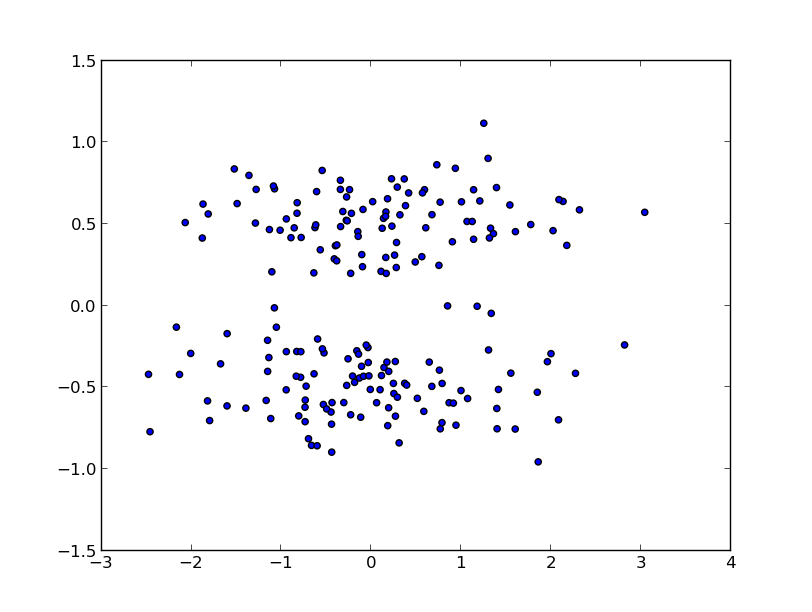
\includegraphics[width=10cm]{images/scatter2Gaussians.png}
	\caption{Scatter plot of the \texttt{2gaussians} data set.}
	\label{fig:scatter2Gaussians}
\end{figure}

\begin{figure}
	\centering
	\subfloat[\label{fig:sub:2GaussiansKM}]{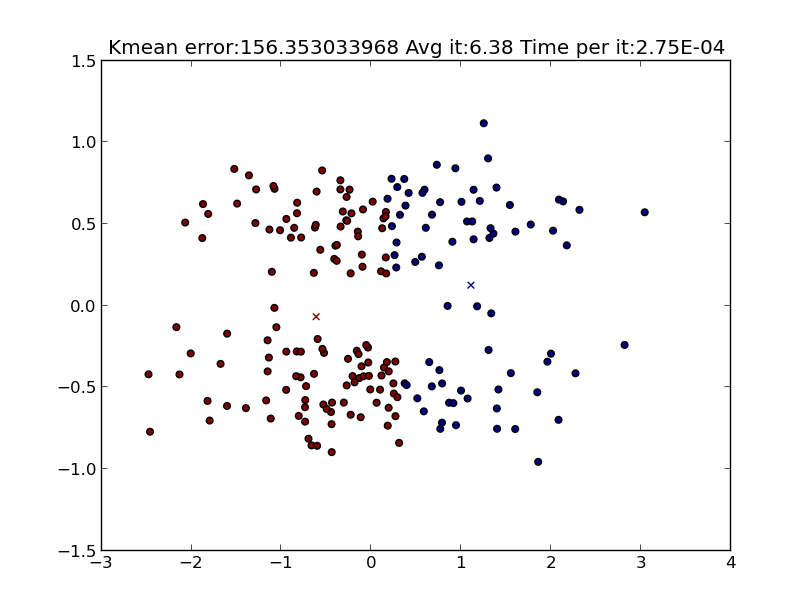
\includegraphics[width=8cm]{images/2gKM.png}}
	\\
	\subfloat[\label{fig:sub:2GaussiansEM}]{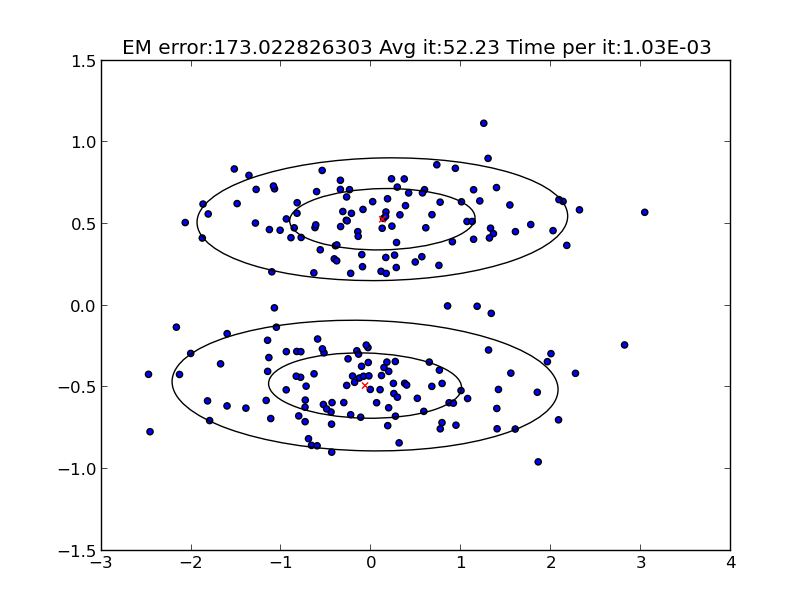
\includegraphics[width=8cm]{images/2gEM.png}}
	\\
	\subfloat[\label{fig:sub:2GaussiansEMKM}]{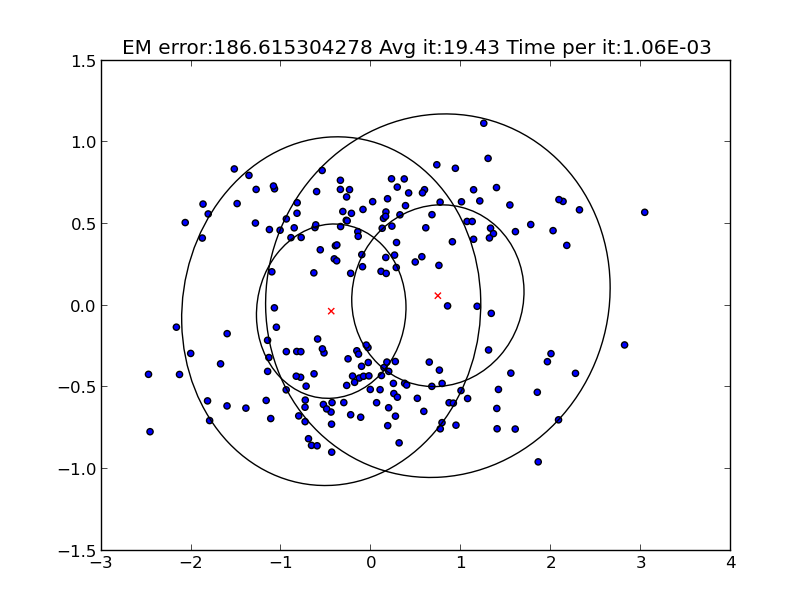
\includegraphics[width=8cm]{images/2gEMkm.png}}
	\caption{Clustering results of the data set \texttt{2gaussians}. \protect\subref{fig:sub:2GaussiansKM} \texttt{k-means}, \protect\subref{fig:sub:2GaussiansEM} \texttt{EM-algorithm} without initialization and \protect\subref{fig:sub:2GaussiansEMKM} \texttt{EM-algorithm} with initialization. } 
	\label{fig:2GaussiansClustering}
\end{figure}

Figure \ref{fig:2GaussiansClustering} shows the results of the clustering algorithms \texttt{k-means} and \texttt{EM-algorithm} with and without initialization.
We can clearly see that \texttt{k-means}, Figure \ref{fig:sub:2GaussiansKM}, fails to cluster the data correctly, because it assumes the data to be circularly located around its cluster center.
However, if the data comes from a Gaussian distribution which is highly stretched, this assumption does not hold anymore.
In contrast, the \texttt{EM-algorithm}, Figure \ref{fig:sub:2GaussiansEM} can correctly model the data set and seems to estimate the covariance matrices correctly as well.
But this only works if the \texttt{EM-algorithm} is not initialized.
If we apply a \texttt{k-means} initialization phase before executing the \texttt{EM-algorithm}, we cannot find the correct clusters, as it can be seen in Figure \ref{fig:sub:2GaussiansEMKM}.
Apparently, the \texttt{EM-algorithm} cannot properly recover from the preadjustment of the initialization phase.

\section{Assignment 8}

In the context of this assignment, I applied \texttt{k-means} and the \texttt{EM-algorithm} with and without initialization to the \texttt{USPS} data set.
The \texttt{USPS} data set contains $16\times 16$ images of hand-written numbers from $0$ to $9$.
The data set contains $2007$ data points.
The maximum iterations was chosen to be $500$ and $100$ for \texttt{k-means} and \texttt{EM-algorithm} respectively.
The regularization constant was set to $\delta=1e-5$ and the termination threshold for the log-likelihood was set to $\epsilon=1e-3$.
Moreover, the algorithms were executed with $k=10$ (number of clusters).
All algorithms are executed $20$ times and the best result with respect to the minimal error and the maximum log-likelihood, respectively, is chosen.

\subsection{Which algorithm delivers better results?}

\begin{figure}
	\centering
	\subfloat[\label{fig:sub:uspsKM}]{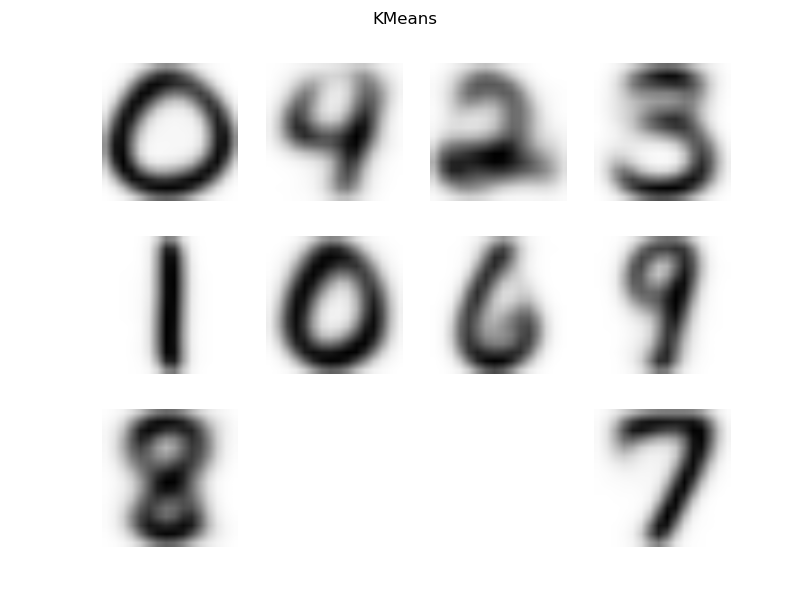
\includegraphics[width=8cm]{images/uspsKM.png}}
	\\
	\subfloat[\label{fig:sub:uspsEM}]{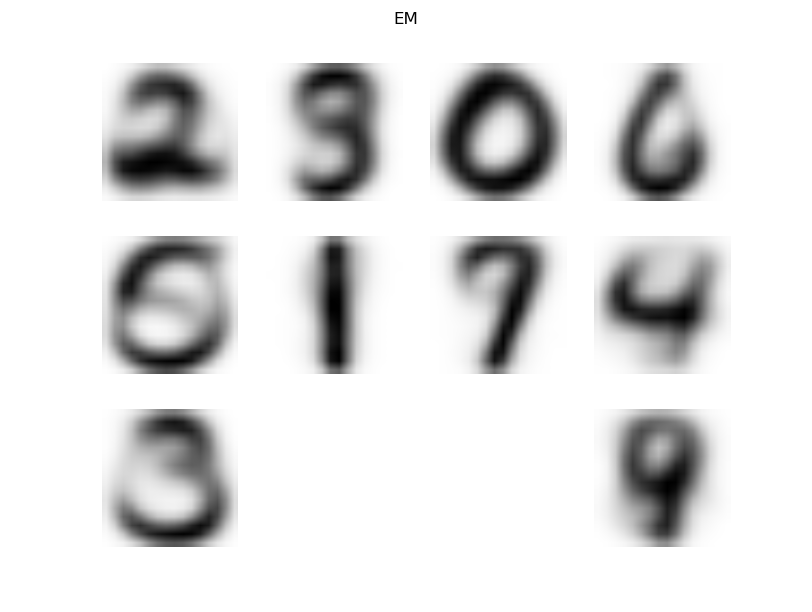
\includegraphics[width=8cm]{images/uspsEM.png}}
	\\
	\subfloat[\label{fig:sub:uspsEMKM}]{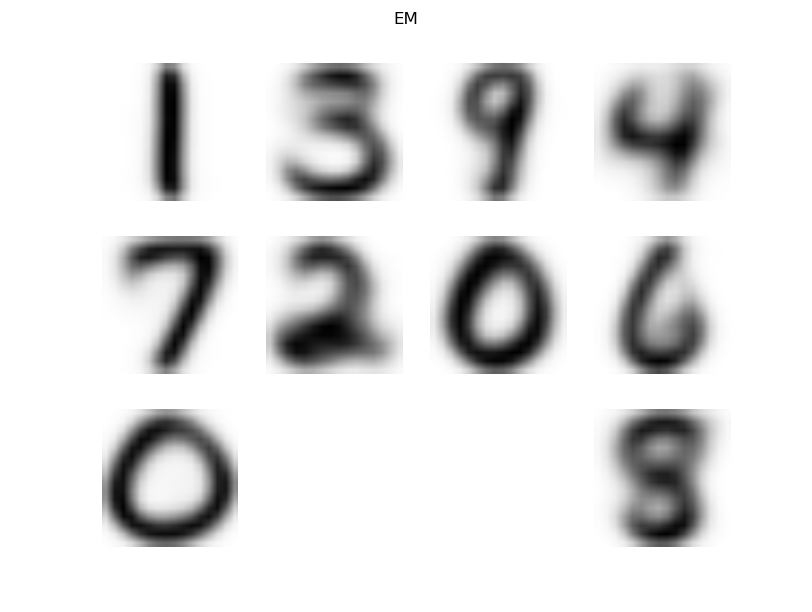
\includegraphics[width=8cm]{images/uspsEMkm.png}}
	\caption{Cluster centroids of the data set \texttt{USPS}. \protect\subref{fig:sub:uspsKM} \texttt{k-means}, \protect\subref{fig:sub:uspsEM} \texttt{EM-algorithm} without initialization and \protect\subref{fig:sub:uspsEMKM} \texttt{EM-algorithm} with initialization. } 
	\label{fig:uspsCentroids}
\end{figure}

Figure \ref{fig:uspsCentroids} shows the centroids of clusters found by \texttt{k-means}, Figure \ref{fig:sub:uspsKM}, by the \texttt{EM-algorithm} without initialization, Figure \ref{fig:sub:uspsEM}, and by the \texttt{EM-algorithm} with initialization, Figure \ref{fig:sub:uspsEMKM}.
Regarding the centroids, one sees that \texttt{k-means} produces the most discriminative centroids.
The only number which is missing is the $5$, because it is usually very similar to the $3$ and thus represented by the centroid of the $3$s.
The \texttt{EM-algorithm} with initialization delivers comparable results which have the same problem with the $5$.
But using this algorithm without an initialization phase produces highly ambiguous centroids, e.g. the $3$ and $8$, $0$ and $5$, $7$ and $9$ are mixed.

\subsection{Dendrogram}

Figure \ref{fig:uspsDendrogram} shows the dendrogram of the hierarchical clustering applied on the \texttt{USPS} data set.
Figure \ref{fig:uspsInitialCentroids} shows the initial centroids found by \texttt{k-means} and which are used for the hierarchical clustering algorithm.

\begin{figure}
	\centering
	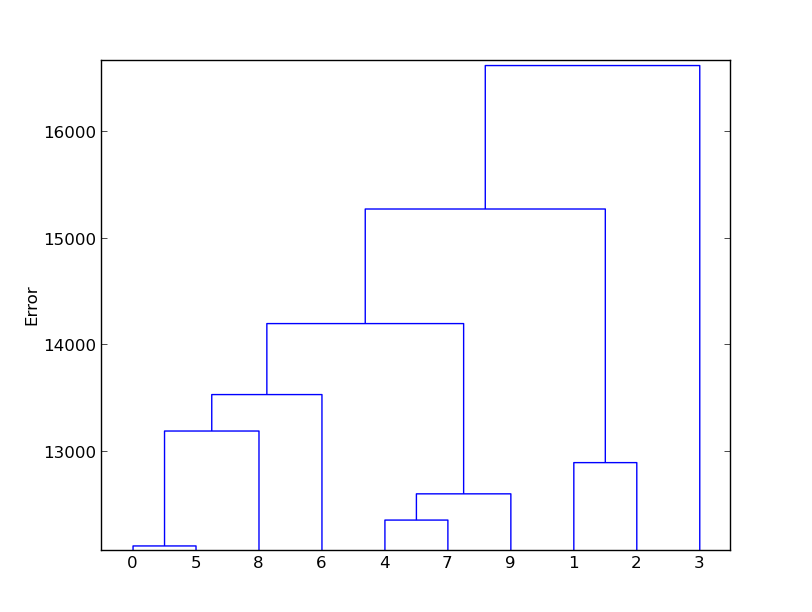
\includegraphics[width=12cm]{images/uspsdendrogram.png}
	\caption{Dendrogram of the hierarchical clustering of data set \texttt{USPS}.}
	\label{fig:uspsDendrogram}
\end{figure}

\begin{figure}
	\centering
	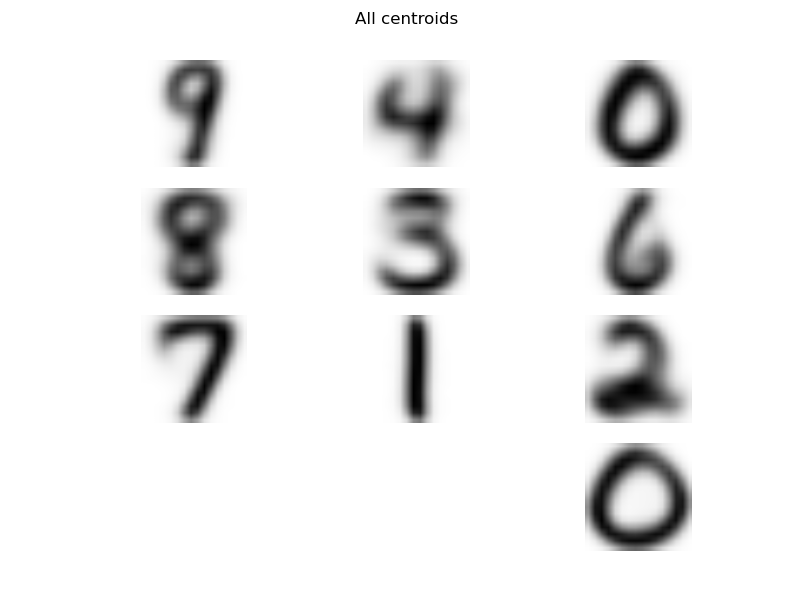
\includegraphics[width=12cm]{images/allcentroids.png}
	\caption{All initial centroids found by \texttt{k-means}.}
	\label{fig:uspsInitialCentroids}
\end{figure}

Figure \ref{fig:uspsMerges} shows in chronological order from left to right and top to bottom the different cluster merges. 
The left and middle image show the centroids of the two clusters chosen to be merged and the right image shows the resulted centroid.
We can see that at first clusters with similar centroids are merged and that at each step the cluster differ a little bit more from each other.
Furthermore, we can observe that the resulting centroid loses more and more its distinctness.
This is not surprising considering the fact that after each merge operation the resulting cluster has to represent more and more different numbers.

\begin{figure}
	\centering
	\subfloat{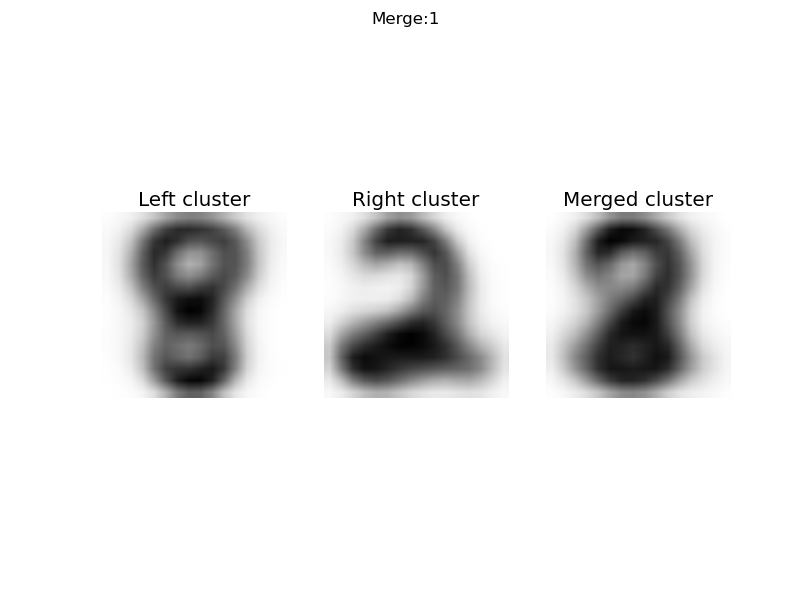
\includegraphics[width=6cm]{images/1merge.png}}
	\subfloat{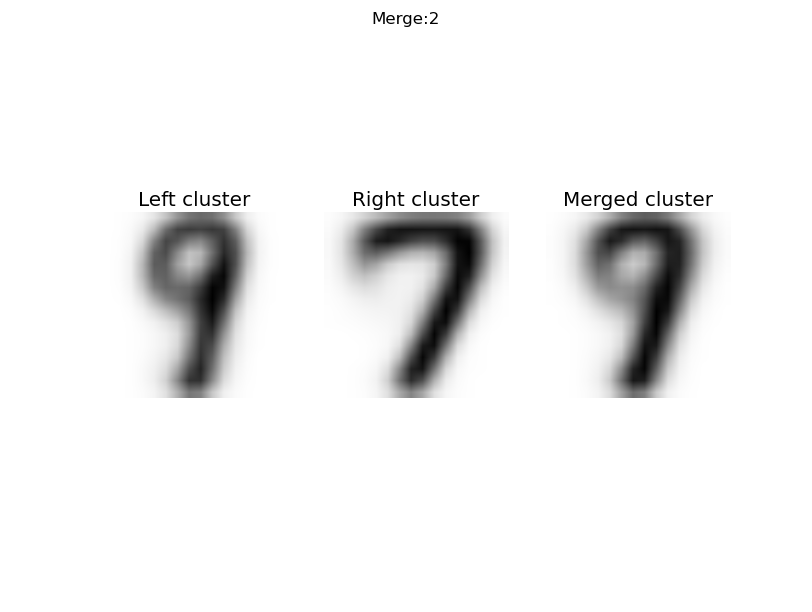
\includegraphics[width=6cm]{images/2merge.png}}
	\subfloat{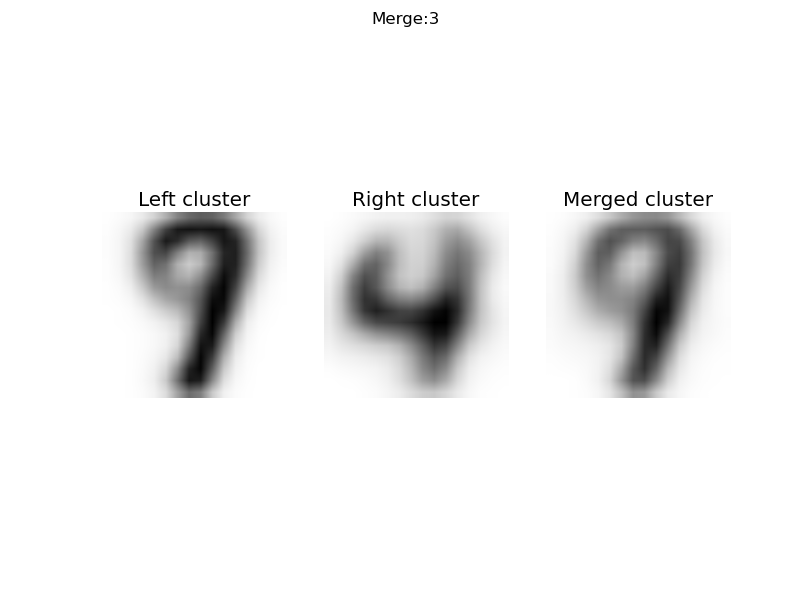
\includegraphics[width=6cm]{images/3merge.png}}
	\\
	\subfloat{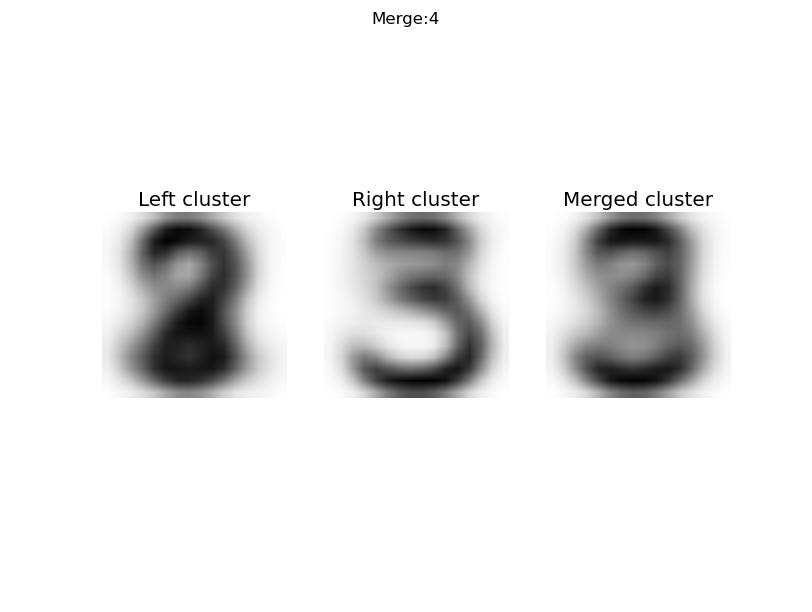
\includegraphics[width=6cm]{images/4merge.png}}
	\subfloat{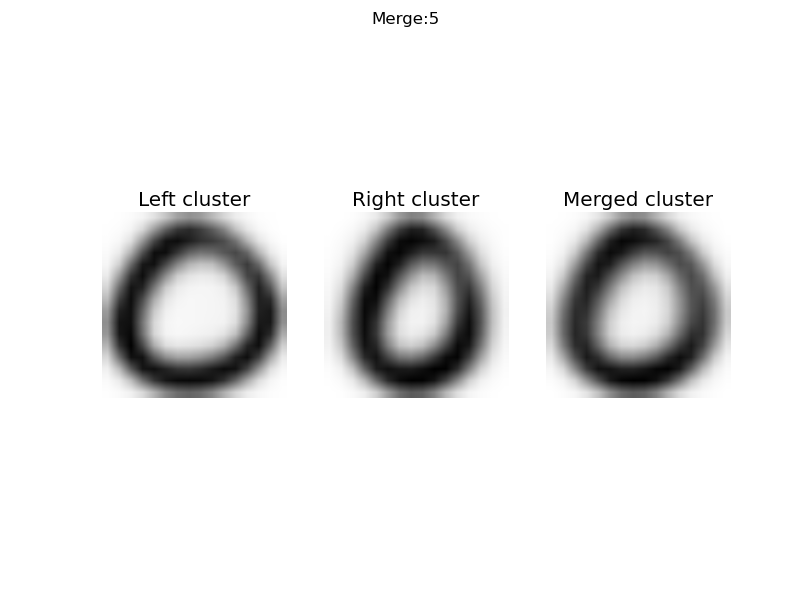
\includegraphics[width=6cm]{images/5merge.png}}
	\subfloat{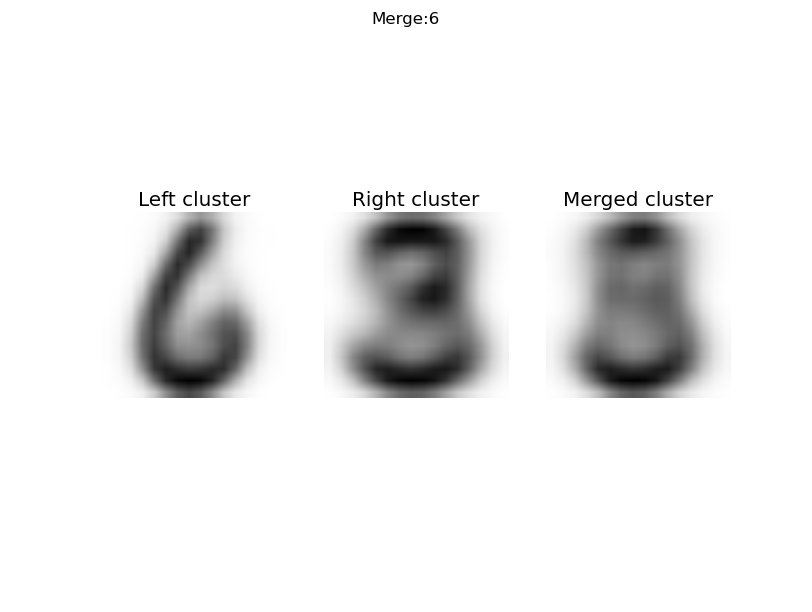
\includegraphics[width=6cm]{images/6merge.png}}
	\\
	\subfloat{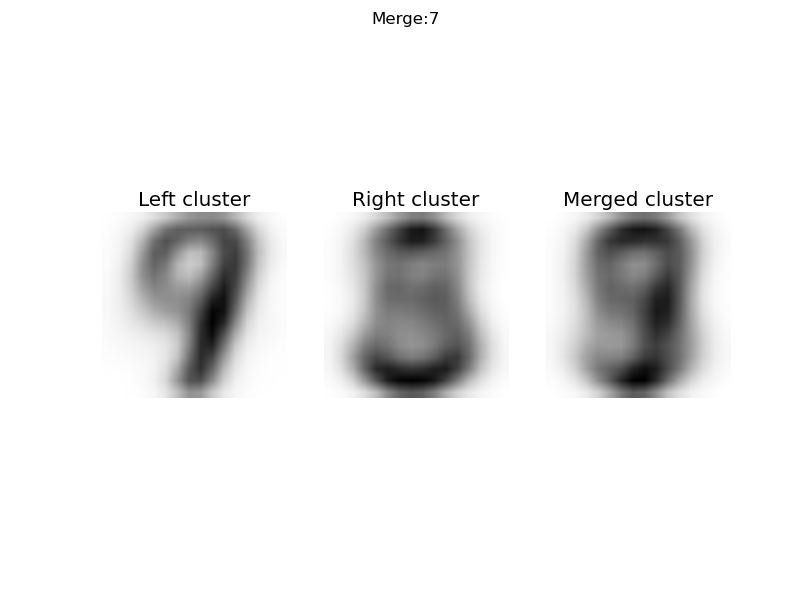
\includegraphics[width=6cm]{images/7merge.png}}
	\subfloat{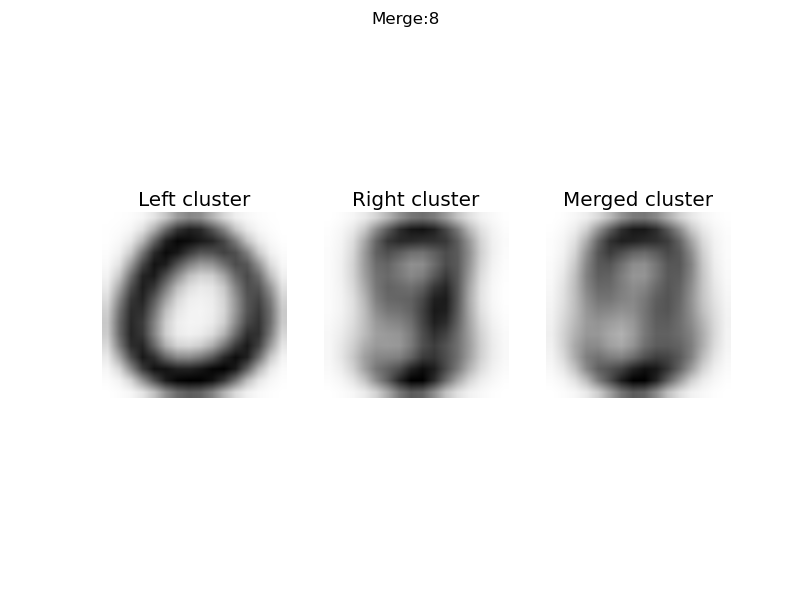
\includegraphics[width=6cm]{images/8merge.png}}
	\subfloat{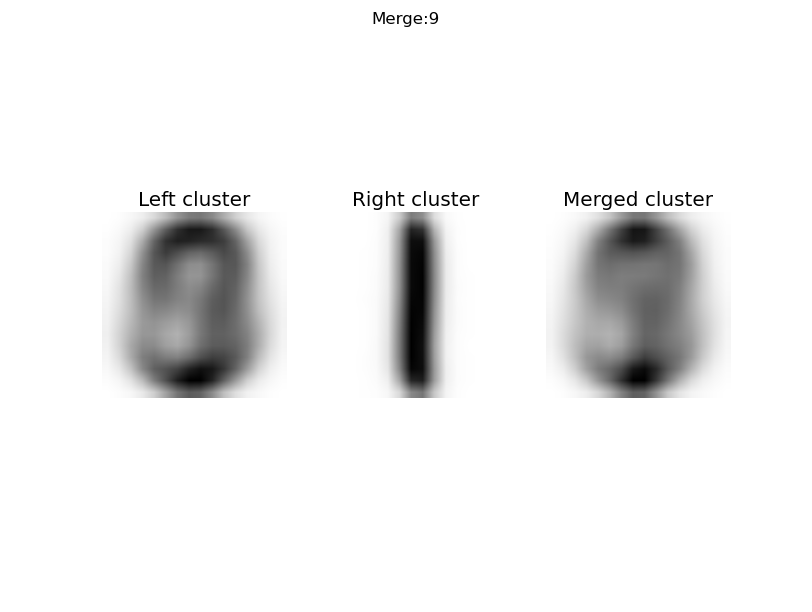
\includegraphics[width=6cm]{images/9merge.png}}
	\caption{Centroids before and after merge operation. From left to right and top to bottom is the chronological order.}
	\label{fig:uspsMerges}
\end{figure}

\end{document}
